\documentclass{article}
\usepackage{nips10submit_e,times}
\usepackage{graphicx}

\title{The Topic Browser\\An Interactive Tool for Browsing Topic Models}
\author{
Matthew J. Gardner \\
Department of Computer Science \\
Brigham Young University \\
Provo, UT 84604 \\
\texttt{mjg82@byu.edu} \\
\And
Other authers\ldots \\
Affiliation \\
Address \\
\texttt{email} \\
}

%\nipsfinalcopy % Uncomment for camera-ready version

\begin{document}
\maketitle

\begin{abstract}

Topic models have been shown to capture a measure of the semantics in a corpus.
Many individualized and cherry-picked visualizations of topic models have been
reported in the literature, showing the potential of topic models to give
valuable insight into a corpus.  However, good, general tools for browsing the
entire output of a topic model along with the analyzed corpus have been
lacking.  We present an interactive tool that incorporates both prior work in
displaying topic models as well as some novel ideas that greatly enhance the
visualization of these models.

\end{abstract}

\section{Introduction}

Proper visualizations are essential to extracting information from and
identifying trends in data, especially large, highly dimensional data.  Large
text corpora are particularly difficult to visualize, as they typically include
thousands of documents and perhaps millions of words.  Topic
modeling~\cite{blei-2003-latent-dirichlet-allocation} is a method of reducing
the dimensionality of a corpus into a set of meaningful topics.  Topic models
have been used with some success as an aid to corpus
visualization~\cite{blei-2009-topic-models,
newman-2010-visualizing-with-topic-maps}.  However, in general the presentation
of topic models has been limited to hand selected topics that show the model in
the best light possible.  These presentations leave the viewer wondering what
else the topic model discovered and provide little help in gaining a deep
understanding of the model.

To aid in the visualization of topic models and in pattern discovery in
document collections, we present The Topic Browser, a tool for interactively
exploring both the output of a topic modeling algorithm and its attendant
corpus.  Our topic browser incorporates many visualizations of topic models
previously published as well as some innovative ideas of our own.  The Topic
Browser is an aid both to those who wish to browse through a corpus and for
those who wish to analyze the topic model itself.

The rest of this paper describes the Topic Browser.  We demonstrate our tool
with a topic model run on a collection of about 460 campaign speeches from the
2008 presidential primary and general elections.

\section{Extra Information}

Aside from the documents and the topic model themselves, our browser
incorporates three other pieces of information: attributes (or metadata)
associated with each document, topic metrics, and document metrics.  Here we
give a brief description of these kinds of information, deferring a discussion
of their use in visualization to the subsequent sections.

Attributes of documents have been used heavily in recent topic models,
including the Author-Topic model~\cite{rosen-zvi-2004-author-topic-model},
Topics over Time~\cite{wang-2006-topics-over-time}, and Dirichlet-Multinomial
Regression~\cite{mimno-2008-topic-models-with-arbitrary-features-dmr}.  While
we currently do not have specialized visualizations for these topic models, we
do include document attributes in our browser and have some of our own 
visualizations that include the attributes.

In order to browse more effectively through topics, we introduce topic metrics
that give information about the topic.  These range from simple metrics, such
as the number of tokens and types labeled with the topic, to more complicated
metrics like how dispersed the topic is across documents, or how coherent its
words are~\cite{newman-2010-automatic-evaluation-of-topic-coherence}.  We also
use pairwise topic metrics as similarity measures to show similar topics.

Similar to topic metrics, one can also compute document metrics.  Beyond simple
metrics like token count in the document, these can include things such as the
entropy of the topic distribution of the
document~\cite{misra-2008-lda-to-find-semantically-incoherent-documents}.  And
as with topics, we make use of pairwise document metrics such as topic
correlation~\cite{blei-2009-topic-models} to show similar documents.

\section{Sidebar}

The sidebar in our browser is the main navigation tool.  Apart from the obvious
task of directing the user to various parts of the visualization tool, the main
purpose of the sidebar is to list the items of a particular type (such as
topics or documents).  The new capability introduced by this browser is the
ability to sort and filter these lists as the user desires.

When presenting the results of a topic model analysis, papers will often
cherry-pick the list of topics looking for particularly good topics to display,
leaving the large number of meaningless topics untouched.  While such
presentations may help the researcher to highlight the benefits of her new
topic model, they hide the fact that finding good topics is often a laborious
process.  With our topic and document metrics, the sorting and filtering
capabilities of the sidebar list allow the user to often go quickly to the very
topics he desires to find.

When browsing through topics, the user can filter the topic list by coherence
to eliminate from the view topics that are mostly meaningless, and sort by
document entropy to find topics that were used widely (or narrowly, if that is
desired) throughout the corpus.  For example, Figure~\ref{fig:sidebar} shows
that the family was one of the most consistent themes in the speeches.

\begin{figure}
  \centering
  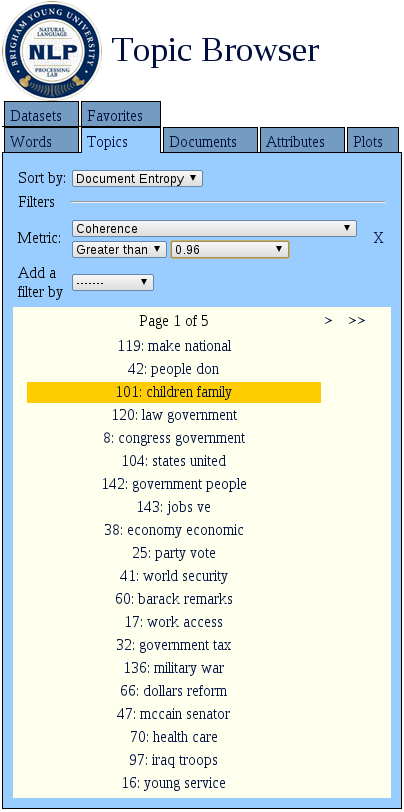
\includegraphics[width=.34\textwidth]{sidebar}
  \caption{The navigational sidebar showing topics sorted by dispersion
  throughout the corpus and filtered by coherence}
  \label{fig:sidebar}
\end{figure}

The user can also filter by document or attribute, seeing only topics that were
used in a particular document or by a particular author.  Documents can
similarly be filtered and sorted, showing only documents that contain tokens
with a particular topic, or with a particular value of an attribute.

\section{Topic Browsing}

Topic models are typically presented as static lists of words, often simply
showing the top ten words from each topic in a list.  While this practice is
often sufficient to give a reader a basic idea of what the topic captured, it
is largely incapable of conveying a deep understanding of the context of that
topic in the corpus.  In order to answer significant questions about a corpus
one must browse the topics discovered, and previous methods have failed to
adequately allow the user to explore topics.  Our browser presents new ways
to gather information about a topic in the corpus, both in how the words in the
topic are displayed and in that is presented about the topic.

\subsection{Showing Top Words}

Instead of showing a list of the top ten words, we show a word cloud of the top
100, where the size of each word is determined by the probability of seeing
that word in the topic.  We also show a re-weighted word cloud as determined by
Blei \& Lafferty's Turbo Topics method~\cite{blei-2009-turbo-topics}.

While these visualizations are modest improvements over typical visualization
methods, our most useful display of the words is showing them in their context.

The topics in a topic model cannot be fully interpreted when completely
separated from their context.  Thus we display the top ten words in the topic
inside of their context.  We select a random token of each word type labeled
with the topic and show up to 50 characters on either side of the token,
keeping words intact.  We also allow the user to cycle through contexts to gain
a broader view of how each word is actually used in that topic in the corpus.
When viewing the topic about troops in Iraq, for example (see
Figure~\ref{fig:context}), one can see that most often when the word ``troops''
is used in this topic, it is in reference to bringing the troops home, and when
``end'' is used, it is not used in the context of ``end the war'' as often as
one might expect.

\begin{figure}
  \centering
  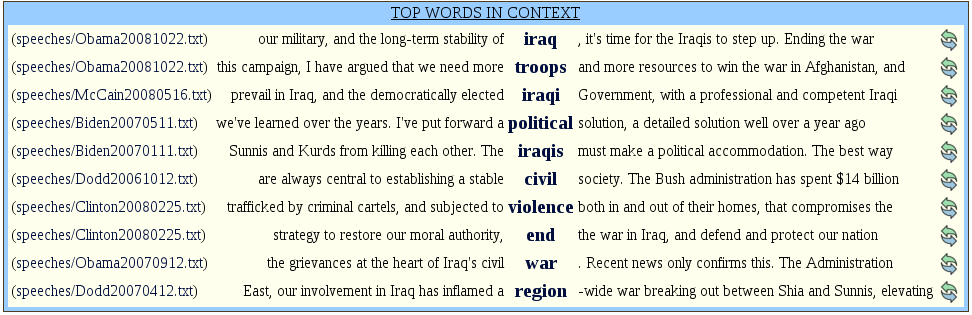
\includegraphics[width=.8\textwidth]{words_in_context}
  \caption{The top ten words in the topic shown with a random context selected
  from the corpus.}
  \label{fig:context}
\end{figure}

\subsection{Getting More Information}

The browser provides two main ways of getting more information about topics in
the model.  The first is showing documents and attribute values which have
either the highest number of tokens labeled with that topic or the highest
proportion (by percentage) of the given topic.  This allows the user to quickly
find documents that best demonstrate what the topic captured.  Showing the top
values for a given attribute (such as authors for the attribute ``Author'')
gives the user an idea of how focused the topic is and often gives interesting
information about the corpus being browsed.  For example, in Figure
\ref{fig:top-values}, we see that Democrats spoke more often about education
than Republicans did, at least in the topic shown.

\begin{figure}
  \centering
  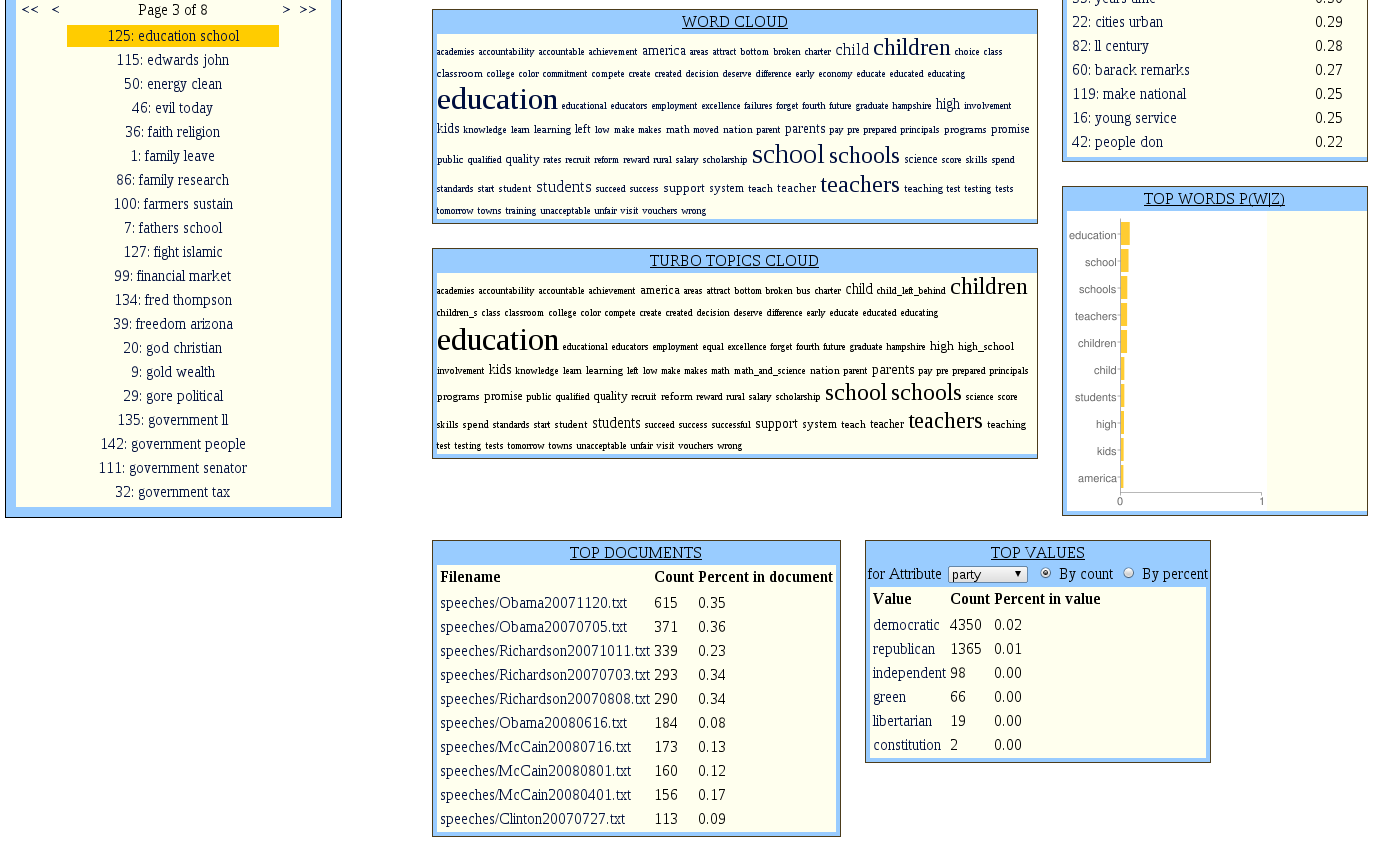
\includegraphics[width=\textwidth]{top_values}
  \caption{Part of the overall topic view, looking at a topic about education.
  Note particularly the top documents for the topic and the top values for the
  attribute ``party,'' shown at the bottom.}
  \label{fig:top-values}
\end{figure}

The other way that we give more information about topics is by showing similar
topics.  We find similar topics either by looking at the documents that the
topics show up in or by the words that the topics use.  Looking at similar
topics by document shows topics that are commonly used together in the corpus,
and looking by word shows topics that have similar words, possibly because the
two topics really should have been one topic.  When looking at a topic about
health care, the user can see that other topics used together with the health
care topic include topics about the cost of medication and the quality of care
(see Figure~\ref{fig:similar}).

\begin{figure}
  \centering
  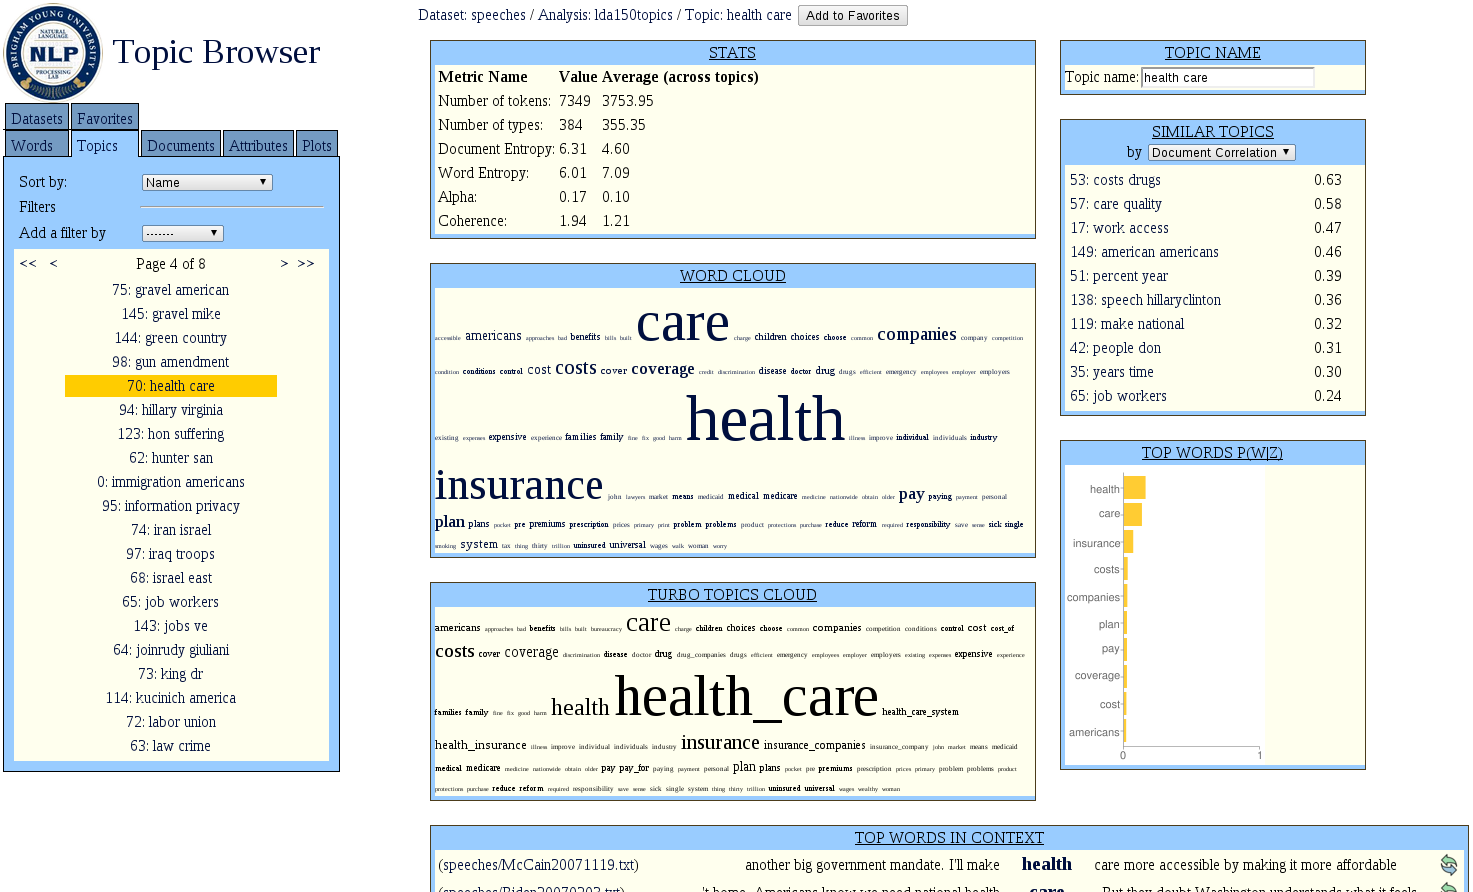
\includegraphics[width=\textwidth]{similar_topics}
  \caption{Another look at the overall topic view, featuring different parts of
  the view.  Note particularly the similar topics box near the top right.}
  \label{fig:similar}
\end{figure}

\section{Document, Word, and Attribute Browsing}

In addition to enabling the user to browse the topics in the topic model, we
provide means for browsing the documents, words, and attributes in the corpus.
These facilities give users means to explore the corpus itself in the context
of the topic model.

When simply browsing through the documents, we provide sorting and filtering
methods on the list of documents, as mentioned previously.  When looking at a
particular document, we show basic information about the document, its text,
the topic distribution in the document, and similar documents based on that
distribution.  When looking at the document in the context of a topic, we also
highlight the tokens in the document that were labeled with that topic.  For
example, the user might be curious to see a document that best demonstrates the
health care topic mentioned above.  Clicking on the top document in the document list brings the user to the view shown in Figure~\ref{fig:document}.

\begin{figure}
  \centering
  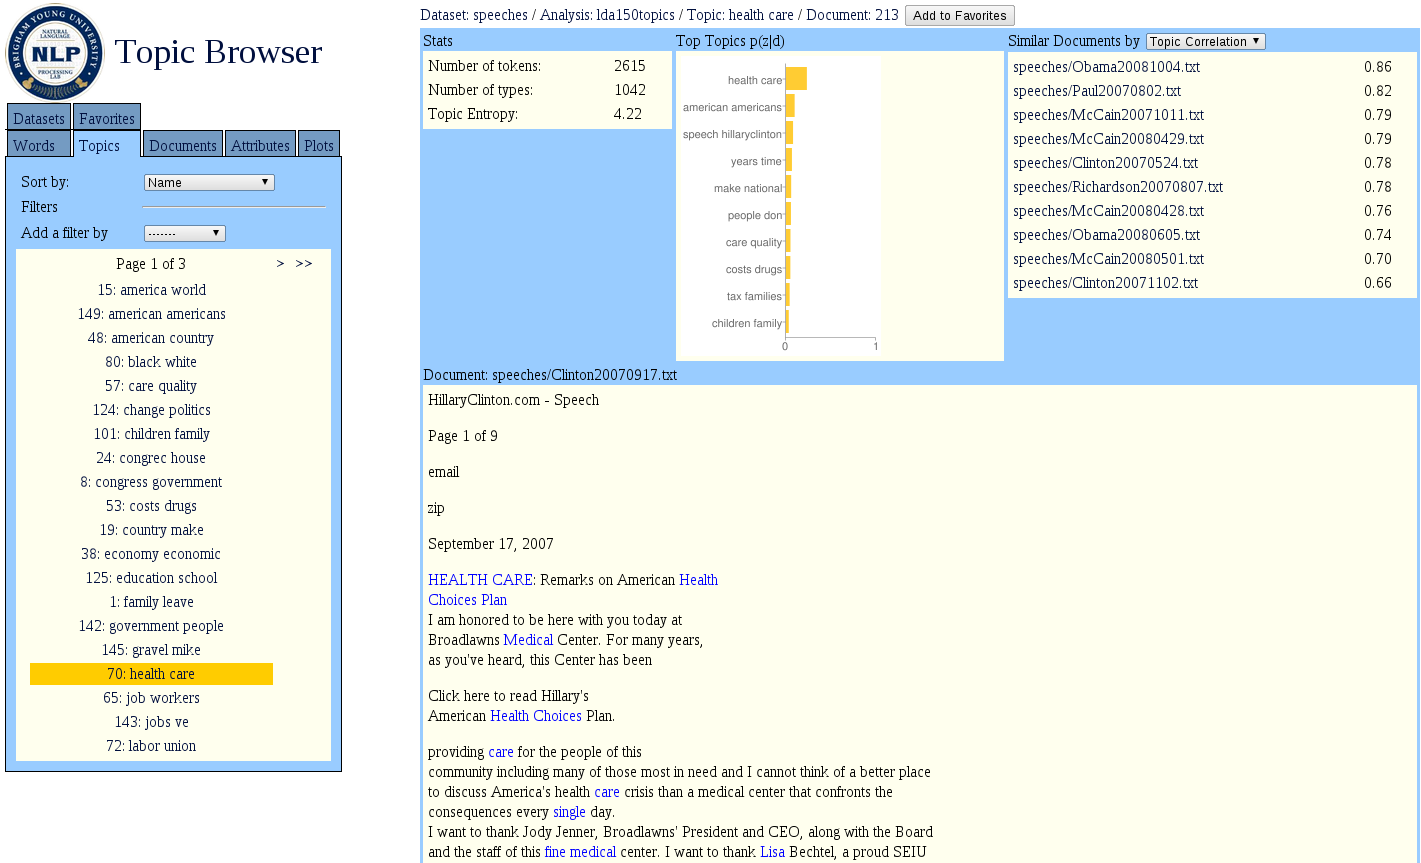
\includegraphics[width=\textwidth]{document}
  \caption{The document view, looking at a speech by Hillary Clinton in the
  context of a topic about health care (the rest of the document is cut off in
  this screenshot).}
  \label{fig:document}
\end{figure}

These document visualizations been done previously, and in fact the view in
Figure~\ref{fig:document} constitutes the entirety of most previous corpus
browsers based on topic models.  This functionality is all that is generally
provided in other browsers, though it is just a small part of ours.

We also provide views of individual words in the corpus.  When viewing a word
in the context of a topic, the user can see all uses of the word in that topic
in the corpus, with context taken from their corresponding documents.  The user
can also view words independently with a search-like interface, seeing topics
and documents in which the word appears most frequently.  The user examining
the health care topic might be curious where else the word ``health'' was used
in the topics and the corpus.  Figure~\ref{fig:word} shows the result of using
our word search to answer that question.  While providing basic functionality,
however, the search interface leaves much to be desired, as only single words
can currently be searched for.  We plan on expanding that to phrases.

\begin{figure}
  \centering
  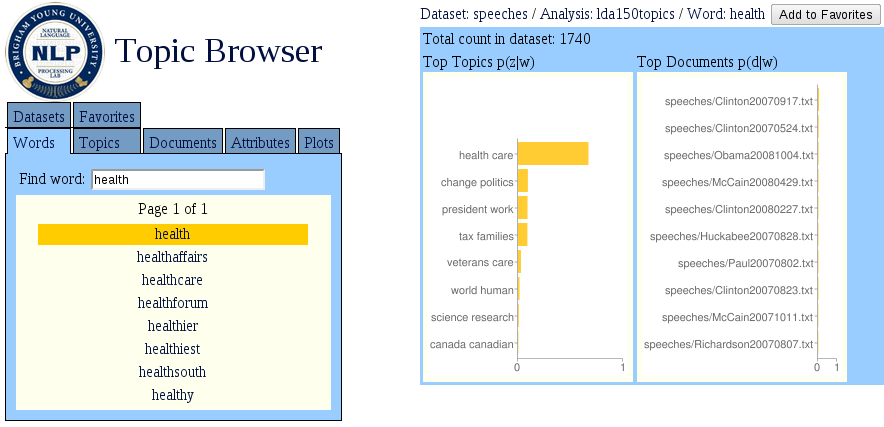
\includegraphics[width=.72\textwidth]{word}
  \caption{The word search functionality, showing the results for searching for
  the word ``health.''}
  \label{fig:word}
\end{figure}

The user can also look at aggregated information for values of an attribute
(i.e., a particular author or year in the documents), combining all of the
topic and word counts for all documents with the given attribute.  This view is
also at present somewhat limited, showing only what topics and words are used
most frequently by the collection of documents with that attribute.
Figure~\ref{fig:attribute} shows us, among other things, that one of Barack
Obama's top topics was change in politics.

\begin{figure}
  \centering
  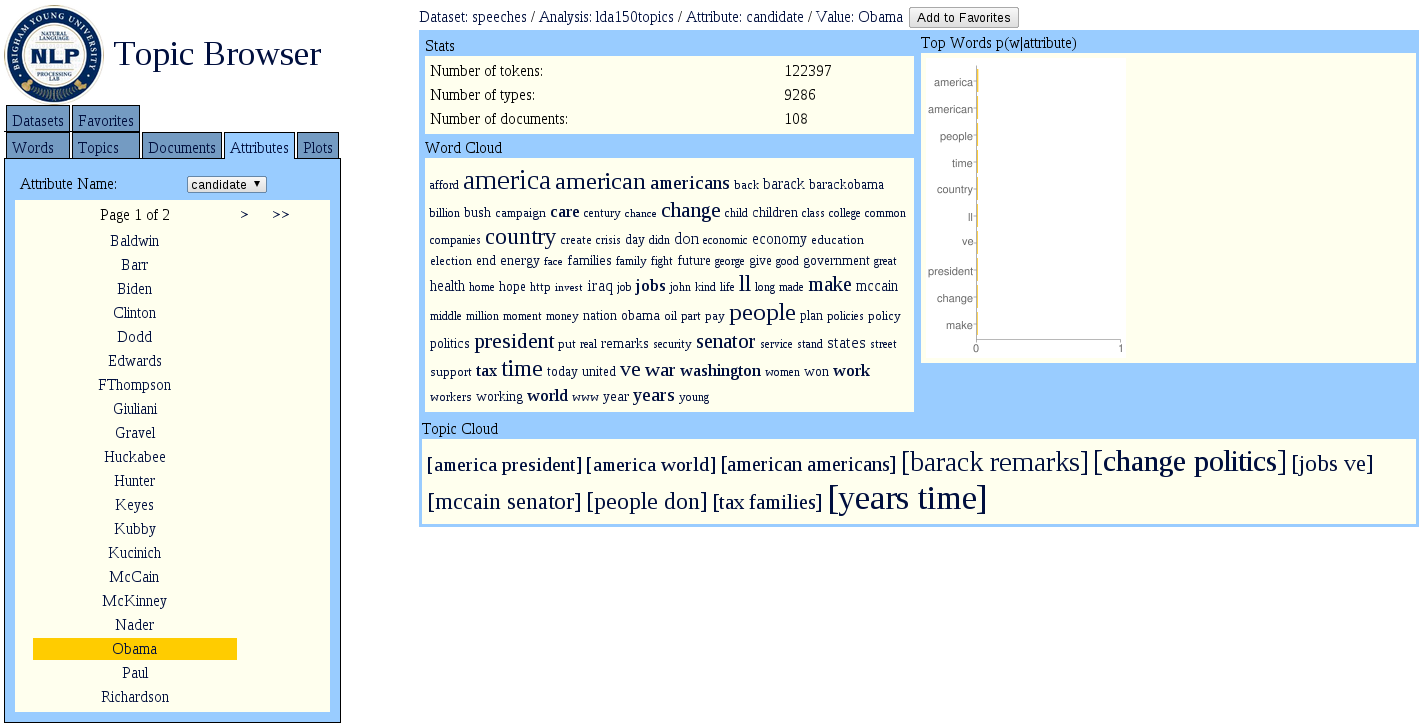
\includegraphics[width=\textwidth]{attribute}
  \caption{The attribute view, showing aggregated information for all speeches
  given by Barack Obama.}
  \label{fig:attribute}
\end{figure}

\section{Plots}

We currently include two kinds of plots in our topic browser, with plans to
implement many more.  The first is showing trends for topics over the values of
an attribute (such as date, or author), useful for corpus browsing.  This kind
of plot has been used in visualizing topic models almost since their
introduction~\cite{griffiths-2004-finding-scientific-topics}.  Our topic
browser allows the user to interactively generate these trend plots over any
attribute for any topic or combination of topics of the documents in the
corpus.  Our user exploring health care topics may want to view how much each
candidate spoke about health care.  We saw already that there were three
related topics that mentioned health care, so the user views all of them
together in a histogram, shown in Figure~\ref{fig:trend-plot}

\begin{figure}
  \centering
  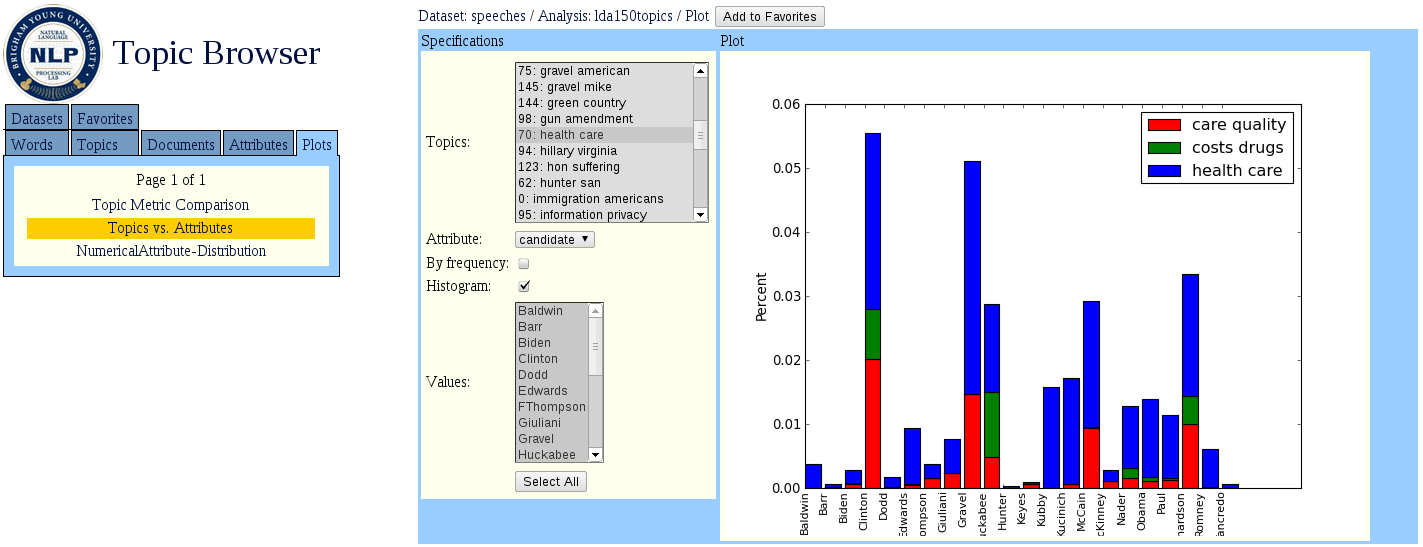
\includegraphics[width=\textwidth]{trend_plot}
  \caption{A plot of topics over attributes, showing the use of three health
  care-related topics across candidates.}
  \label{fig:trend-plot}
\end{figure}

The second kind of plot that we include is more useful for analyzing and
understanding the behavior of the topic model itself.  We allow the user to
plot two topic metrics against each other and compute a linear regression.
This allows the user to see some interesting properties of the topic metrics,
such as the fact that document entropy seems to correlate with the logarithm of
the number of tokens in the topic, and that coherence does not seem to
correlate with any other topic metric.  The user can also find outliers, such
as topics with low document entropy but a high token count, that can then be
examined in the topic page.

An interesting application of these topic metric plots occurs when the metrics
include how consistently each candidate spoke about each topic.
Figure~\ref{fig:metric-plot} shows a plot of topics, comparing John McCain's
use of the topic to Barack Obama's use of the topic.  Topics in the upper left
were topics unique to Obama, and topics in the lower right were unique to
McCain.  Topics in the middle (near the value of 2 for each candidate) were
somewhat shared between the two.

\begin{figure}
  \centering
  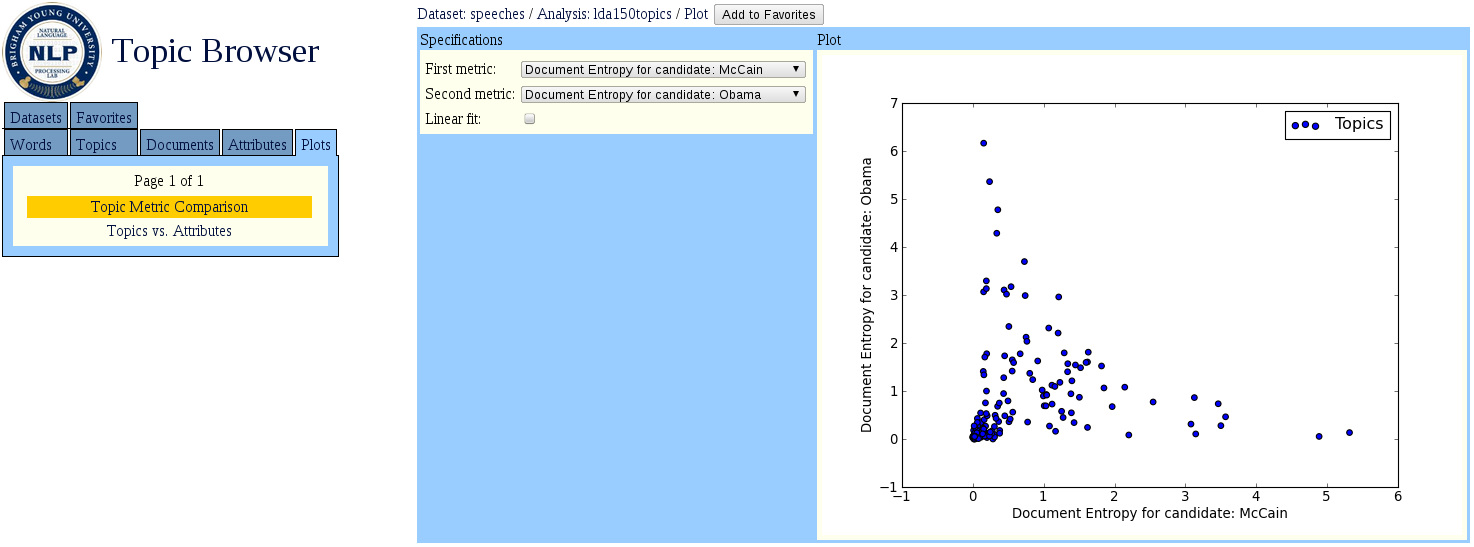
\includegraphics[width=\textwidth]{metric_plot}
  \caption{A topic metric comparison plot.  The metrics used were how
  consistently Barack Obama and John McCain used each topic. The plot shows
  topics that were unique to Obama or McCain and topics they shared.}
  \label{fig:metric-plot}
\end{figure}

\section{Conclusion}

We have presented the Topic Browser, an interactive tool for browsing both the
output of a topic model and the corpus that was modeled.  We have shown that
our tool incorporates many previously published visualizations of topic models,
including basic corpus browsing functionality, plots of trends over attributes
in the corpus, and Blei \& Lafferty's Turbo Topics method of finding
significant phrases for each topic.  We have also presented many novel ways to
mine information from a topical analysis of a corpus in an interactive browsing
experience.

While our tool is still under development, we intend to make it open and freely
available, both for those wishing to browse through a corpus in the context of
a topic model, and for those wishing to better understand topic models and
develop new models.  Our tool currently supports any topic model that labels
individual tokens in the corpus with topics.  We have plans to include special
visualizations for more complicated topic models, such as Topics over Time,
sentiment-topic models, hierarchical topic models, and others.

\bibliographystyle{plain}
\bibliography{../../../bib/lda/bib}

\end{document}
